%%%%%%%%%%%%%%%%%%%%%%%%%%%%%%%%%%%%%%%%%%%%%%%%%%%%%%%%%%%%%%%%%%%%%%%%%%%%
%% Trim Size : 11in x 8.5in
%% Text Area : 9.6in (include Runningheads) x 7in
%% ws-jai.tex, 26 April 2012
%% Tex file to use with ws-jai.cls written in Latex2E.
%% The content, structure, format and layout of this style file is the
%% property of World Scientific Publishing Co. Pte. Ltd.
%%%%%%%%%%%%%%%%%%%%%%%%%%%%%%%%%%%%%%%%%%%%%%%%%%%%%%%%%%%%%%%%%%%%%%%%%%%%
%%

%\documentclass[draft]{ws-jai}
\documentclass{ws-jai}
\usepackage[flushleft]{threeparttable}
\usepackage{siunitx}
\usepackage{amsmath}
\usepackage{gensymb}
\usepackage[colorlinks=true,allcolors=blue]{hyperref}
\usepackage{graphicx}
\usepackage{caption}
\usepackage{subcaption}
\usepackage[bottom]{footmisc}
\usepackage{url}

% Define stuff here
\def\albatros{ALBATROS}
\def\prizm{PRI$^{\rm Z}$M}

\begin{document}

\catchline{}{}{}{}{} % Publisher's Area please ignore

\markboth{Author's Name}{ALBATROS instrument}

\title{The Array of Long-Baseline Antennas for Taking Radio
  Observations from the Sub-Antarctic}

\author{First Author$^{2}$, Second Author$^{3}$, Third Author$^{3}$ and Fourth Author$^{4}$}

\address{
$^{2}$Department, University Name, City, State ZIP/Zone, Country, fauthor@university.com\\
$^{3}$Group, Company, Address, City, State ZIP/Zone, Country\\
$^{4}$Group, Company, Address, City, State ZIP/Zone, Country, fauthor@company.com
}

\maketitle

\corres{$^{2}$Corresponding author.}

\begin{history}
\received{(to be inserted by publisher)};
\revised{(to be inserted by publisher)};
\accepted{(to be inserted by publisher)};
\end{history}

\begin{abstract}
\textcolor{red}{\bf text to be overhauled later...} \\
The low frequency radio astronomy has the highest potential in
discovering the history of the Universe, this includes observations
of the first stars and the mapping of dark ages. The Array of Long
Baseline Antennas for Taking Radio Observations from the
Sub-Antarctic (ALBATROS) is a new interferometric array. It consists
of autonomous antenna stations that will map the low-frequency sky
from Marion Island. One autonomous station was deployed in Marion
Island in April 2019. The operating frequency range is
\SIrange{1.2}{81}{\MHz} with baselines of $\approx \SI{20}{\km}$. A
two element pathfinder was deployed in Marion Island in April
2018.
\end{abstract}

\keywords{cosmology: observations; dark ages; instrumentation: interferometers}

\textcolor{red}{\bf Open task for any/all: fix references, make a proper bibtex file}

\section{Introduction}

Measurements of redshifted \SI{21}{\cm} emission of neutral hydrogen
across a wide range of radio frequencies have the potential to
elucidate the universe's history from the cosmic ``dark ages'' up to
the formation of large-scale structures (see,
e.g.,~\citep{ska_physics,2013PhRvD..87d3002L,2014ApJ...782...66P}.
The dark ages, which occurred after recombination and correspond to a
period when the universe was filled with neutral hydrogen, are
unexplored to date and represent one of the final observational
frontiers in cosmology.  This epoch contains a potential wealth of
cosmological information~\citep{loeb_zaldarriaga, 2019arXiv190710853C,
  2019arXiv190804296K}, but the required redshifted frequencies of
$\lesssim 30$~MHz are exceptionally difficult to observe.  The primary
experimental challenges include Galactic foreground emission,
ionospheric interference, and terrestrial radio-frequency interference
(RFI).

Very few experiments have measured the radio sky at $\lesssim 30$~MHz.
Comprehensive reviews exist elsewhere (\textcolor{red}{\bf find a good
  reference}), and here, we highlight only a few specific examples.
At the very lowest frequencies, the state of the art among
ground-based measurements dates from the 1950s, when Reber and Ellis
caught brief glimpses of the $2.1$~MHz sky at $\sim
5$\degree\ resolution, using an array of 192~dipoles~\citep{reber,
  article, 1988A&A...195..372W}.  A few space-based missions have also
performed measurements at similarly low frequency ranges; for example,
the Radio Astronomy Explorer-2 operated at \SIrange{0.025}{13}{\MHz}
with $\sim 10$\degree\ resolution at
\SI{4.7}{\MHz}~\citep{1975A&A....40..365A}.  Measurements with
resolution finer than few-degree scales exist only at higher
frequencies.  For example, the Dominion Radio Astrophysical
Observatory surveyed the northern sky at \SI{22}{\MHz} with
\SIrange{1.1}{1.7}{\degree} resolution~\citep{1999A&AS..137....7R},
and most recently, the Owens Valley Long Wavelength Array mapped the
sky with \SI{15}{\arcminute} resolution between 36.528~MHz and
73.152~MHz~\citep{2018AJ....156...32E}.  Although this experimental
list is not comprehensive, it does illustrate the dearth of
information about the $\lesssim 30$~MHz sky and the lack of high
resolution measurements at the lowest frequencies.

\textcolor{red}{\bf More text about the science case, including
  Galactic astrophysics (Jon? Jeff?)}

Preliminary observations from Marion
Island~\citep{2019JAI.....850004P} suggest that despite the
present-day RFI environment, low-frequency observations may still be
accessible from carefully selected locations and with new technology
developments.  In this paper, we present the Array of Long Baseline
Antennas for Taking Radio Observations from the Sub-Antarctic
(\albatros), a new experimental effort that aims to map the
low-frequency sky using an array of autonomous antenna stations.  We
describe the overall instrument design and preliminary measurements
from engineering runs that were performed on Marion Island during
2018--2019.

\section{ALBATROS overview}

\begin{figure}
  \begin{center}
    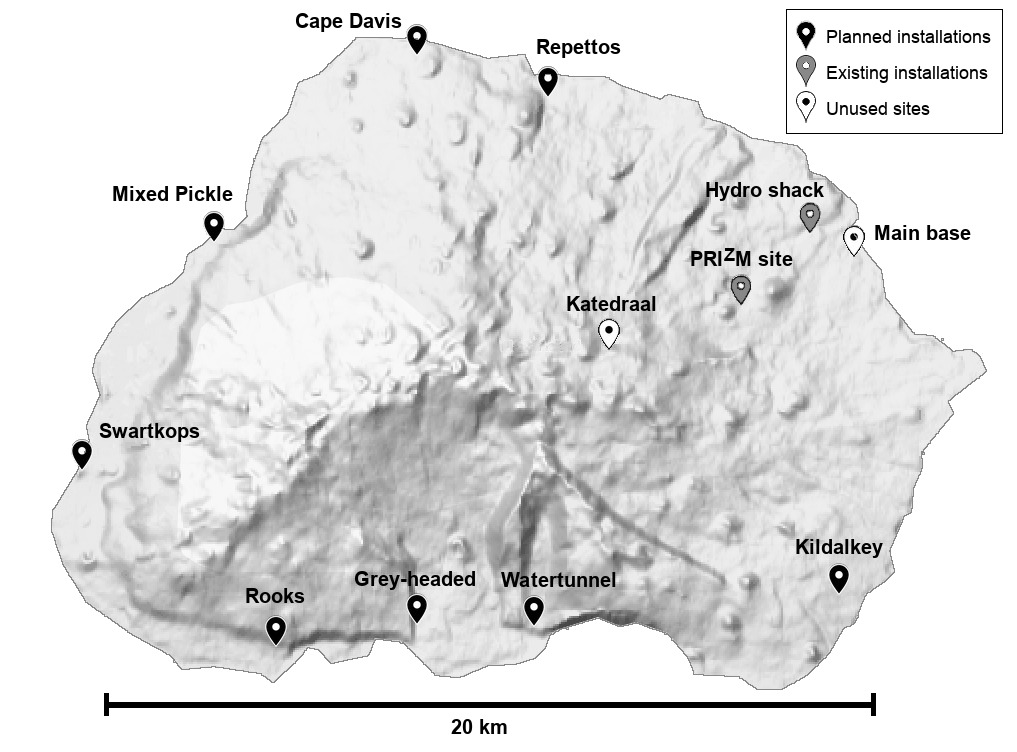
\includegraphics[width=0.7\linewidth]{Figures/marion_map/marion_map_annotated.jpg}
    \caption{Map of Marion Island.  The \albatros\ pathfinder antennas
      are currently installed at the \prizm\ site and at the hydro
      shack.  The black markers denote the eight coastal huts, which
      will be used for future \albatros\ antenna installations.  The
      white markers denote other available infrastructure points that
      will not be used for antennas.  \textcolor{red}{\bf Add new
        synthesized beam figure (Jon)}}
    \label{Fig:marion}
  \end{center}
\end{figure}

% Write text here about the overall final configuration.  Describe the
% site, show synthesized beam, discuss high level system requirements
% (power, data storage, etc).  Include deployment schedule and introduce
% 2-element pathfinder in the following section.

The primary requirements that drive the design for a low-frequency
imaging experiment are 1) desired resolution, 2) low RFI, and 3) quiet
ionospheric conditions.  As a benchmark, an interferometer operating
at 30~MHz requires order-of-magnitude baseline lengths of $\sim 1$~km
to achieve a resolution of $\sim 1$\degree.  This length scales
inversely with frequency, and therefore $\sim 10$-km lengths are
required at few-MHz frequencies in order to improve upon the
resolutions achieved to date.  The experiment installation site must
be remote to keep RFI to a minimum, and polar or near-polar latitiudes
generally have lower ionospheric plasma frequency cutoffs.
\textcolor{red}{\bf Add more ionosphere text here, plus IRI simulation
  fig/numbers (Jon)}

Marion Island is a research base that is located in the southern
Indian Ocean at \ang{46;54;45}S, \ang{37;44;37}E and is operated by
the South African National Antarctic Programme.  The island lies
roughly \SI{2000}{\kilo\metre} from the nearest continental landmasses
and has an exceptionally quiet RFI
environment~\citep{2019JAI.....850004P}.  As illustrated in
\autoref{Fig:marion}, Marion has an area of 335~km$^2$ and can
therefore support antenna installations with $>10$-km baseline
lengths.  The main Marion base is located on the northeast side of the
island, and there are eight rest huts along the coast (Cape Davis,
Grey-headed, Kildalkey, Mixed Pickle, Repettos, Rooks, Swartkops,
Watertunnel) and one in the interior (Katedraal) that can serve as
existing infrastructure points for antenna installations.  The planned
\albatros\ installation sites include the coastal huts, but exclude
the main base and Katedraal for RFI and accessibility reasons,
respectively.  \autoref{Fig:marion} also shows the locations of the
\albatros\ pathfinder antennas that are currently installed at the
\prizm\ site and at the hydro shack.

Using the eight coastal huts, the \prizm\ site, and the hydro shack as
the nominal \albatros\ installation locations, the computed
synthesized beam is as shown in \autoref{Fig:marion}.  The beam width
at 5~MHz is roughly \SI{8}{\arcminute}, which represents over an order
of magnitude improvement in resolution over other existing
measurements.  One of the challenges in constructing an interferometer
array on Marion Island is that the rugged terrain precludes the
possibility of directly cabling and correlating antennas across large
distances.  The final \albatros\ antenna stations will therefore
operate {\it autonomously}, recording baseband data over extended
periods of time for subsequent offline correlation.  We have conducted
two enginering runs: 1) a two-element, directly correlated pathfinder
to qualitatively understand the sky signal, and 2) a single station to
test the readout and power handling technology that are required for
autonomous operation.

\section{Two-element pathfinder}

\begin{figure}
  \begin{center}
    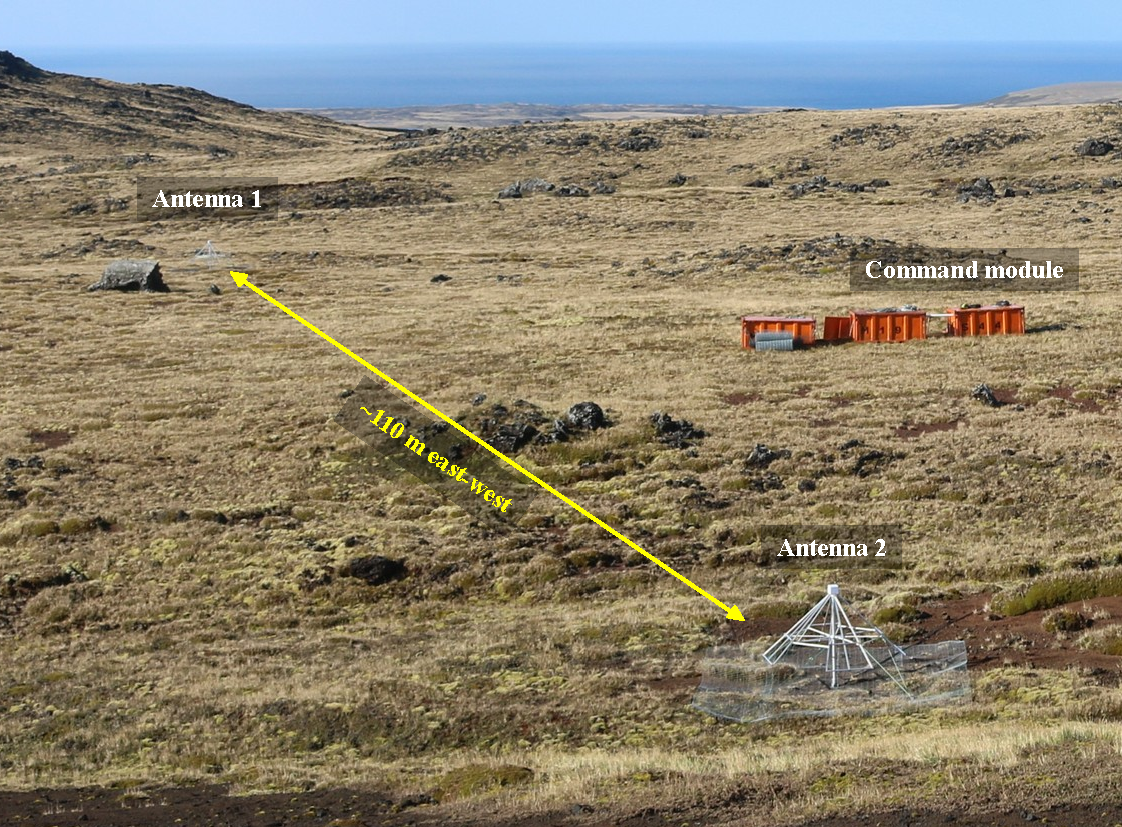
\includegraphics[width=0.7\linewidth]{Figures/albatros_2elem/albatros_2elem.pdf}
    \caption{The two-element, directly correlated
      \albatros\ pathfinder installed at the \prizm\ site.  Two
      dual-polarization antennas are separated by roughly 110~m on an
      east--west baseline. Coaxial cables connect the antennas to a
      shipping container that houses the readout electronics and
      serves as the ``command module.'' \textcolor{red}{\bf Add FEE
        and backend sub-pics here? (HCC)}}
    \label{Fig:albatros2}
  \end{center}
\end{figure}

\begin{figure}
  \begin{center}
    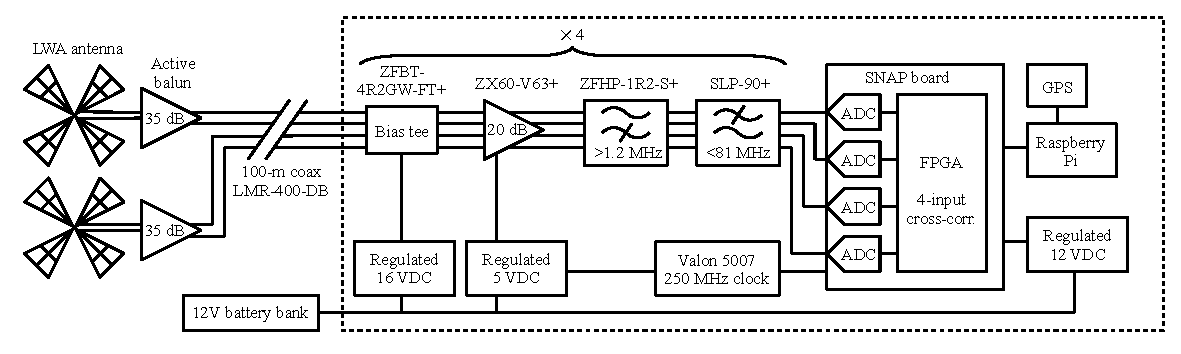
\includegraphics[width=1.0\linewidth]{Figures/albatros_2elem_schematic/albatros_2elem_schematic.pdf}
    \caption{Schematic for the two-element \albatros\ pathfinder.
      Signals from two dual-polarzation LWA antennas are amplified by
      front-end active baluns (\textcolor{red}{\bf citation for FEE}),
      and 100-m coaxial cables connect the antennas to the back-end
      readout electronics, which are housed in a Faraday cage denoted
      by the dashed box.  Each of the four antenna outputs is passed
      to a second-stage electronics chain consisting of a bias tee,
      amplifier, and high- and low-pass filters.  The signals are
      digitized at 250~Msamp/s by a SNAP board, and the on-board FPGA
      is programmed with firmware to perform a full cross-correlation
      of all four inputs.  A Raspberry Pi controls the SNAP board and
      also saves the computed spectra to an SD card.  The clock signal
      is provided by a Valon frequency synthesizer.  Power to the
      system is provided by a bank of 12~V batteries and several
      regulated voltage outputs.}
    \label{Fig:albatros2_schem}
  \end{center}
\end{figure}

The first exploratory \albatros\ measurements were conducted with a
two-element pathfinder that employed direct correlation (without
autonomous operation).  \autoref{Fig:albatros2} illustrates this
pathfinder, which was installed at the \prizm\ site (\ang{46;53;13}S,
\ang{37;49;10.7}E) in April 2018.  The system schematic is illustrated
in \autoref{Fig:albatros2_schem}, and each of the subsystems is
described in detail below.

\subsection{Antenna}	
We employ two dual-polarization Long Wavelength Array (LWA) dipole
antennas~\citep{Memo28}.  The LWA antennas have a long development
history, are well characterized, and are simple to install and
physically robust.  The antennas form an east--west baseline with a
separation of \SI{110}{m}, and the polarizations are aligned with the
cardinal directions.  Welded wire mesh screens, roughly 3~m on a side,
are installed on the ground below the antennas.
% do we want/need to say anything about the omnidirectional primary beam?

\textcolor{red}{\bf ALL TEXT BELOW HERE NEEDS WORK}

\subsection{Front-end active balun}
\textcolor{red}{\bf Tankiso, Eamon, Jeff?} \\
All the front end components were incorporated for in a double sided
printed circuit board (PCB) as shown in \autoref{Fig:Balun} and the
block diagram is shown in \autoref{Fig:Balun Schematic}. The
Monolithic Microwave Integrated Circuits (MMICs) is the used design
for the PCB. One side of the PCB is populated with components and the
other side is a solid copper ground plane aperiodically stitched to
the grounded copper on the side populated with components. The
receiver system is made up of the active balun, filter and the gain
stage that connects to the \SI{100}{\metre} coaxial cable which is
connected to the back end \cite{2012PASP..124.1090H}.

The input impedance (Z\textsubscript{o}) of \SI{50}{\ohm} is
introduced to the dipole by the active balun. The signal is then fed
through an amplifier which amplifies it by \SI{+24}{\decibel} of
gain. The balanced signal is then converted to unbalanced through a
180 \degree hybrid coupler. The band pass filter (BPF) receives the
single ended signal in order for it to reject all the frequencies
which are not within the range of interest. The signal gets fed to a
second amplifier which again amplies it by \SI{+24}{\decibel} of gain
and the output impedance of the FEE is matched to a \SI{50}{\ohm}
coaxial cable. The bias tee is responsible for providing power to the
FEE and extracts the RF signal by the use of the coaxial cable. This
unit has an overall gain of $\approx$ \SI{35}{\decibel} and an overall
noise figure of $\approx$ \SI{2.7}{\decibel} to $\approx$
\SI{2.9}{\decibel} \cite{Memo35}.

\subsection{Back-end electronics}
\textcolor{red}{\bf Nivek, HCC?} \\

The back-end readout electronics are housed in a Faraday cage that is
located $\sim 100$~m away from the antennas to reduce potential
contamination from self-generated RFI.  Each of the four antenna
signals is passed to a second-stage electronics chain consisting of a
bias tee (Minicircuits ZFBT-4R2GW-FT+), amplifier (Minicircuits
ZX60-V63+), and a pair of high- and low-pass filters (Minicircuits
ZFHP-1R2+ and SLP-90+) that band limit the signal to
1.2--\SI{81}{MHz}.  A Smart Network ADC Processor (SNAP) board
digitizes the RF signals at 250~Msamp/s and calculates a full
cross-correlation of the four inputs, producing four auto- and six
cross-spectra as outputs.  \textcolor{red}{\bf finish merging text
  below into the above paragraph}

\textbf{Bias Tee} - It is used to extract the RF signal from a
\SI{100}{\metre} LMR400 coaxial cable which has a nominal attenuation
of \SI{\approx 0.4}{\decibel/\SI{100}{m}} - \SI{\approx
  3.7}{dB/\SI{100}{\metre}} at \SI{1.2}{MHz} - \SI{81}{MHz}
respectively \footnote{https://www.timesmicrowave.com/documents/resources/LMR-400.pdf}. The
bias tee which is used is the Mini Circuits device ZFBT-4R2GW-FT+
which operates between \SI{0.14}{MHz} - \SI{4200}{MHz}. It has an
insertion loss of \SI{0.16}{\decibel} at centre frequency of
\SI{\approx 10}{MHz} as per the
datasheet \footnote{https://www.minicircuits.com/pdfs/ZFBT-4R2GW-FT+.pdf}.

\textbf{HPF} - The HPF rejects any signals with low frequencies and
allow through signals with high
frequencies \footnote{http://www.learningaboutelectronics.com/Articles/High-pass-filter.php}. The
HPF used is the ZFHP-1R2+ Mini Circuits device which operates between
\SI{1.2}{MHz} - \SI{800}{MHz}. It has a nominal insertion loss of
$\approx$ \SI{0.2}{\decibel} at centre frequency of
\SI{\approx10}{MHz} as per the
datasheet \footnote{https://www.minicircuits.com/pdfs/ZFHP-1R2+.pdf}.

\textbf{LPF} - The LPF rejects all signals with high frequencies and
allows all signals with low
frequencies \footnote{http://www.learningaboutelectronics.com/Articles/Low-pass-filter.php}. The
LPF used is the SLP-90+ Mini Circuits device which operates between
\SI{1}{MHz} - \SI{400}{MHz}. It has a nominal insertion loss of
$\approx$ \SI{0.14}{\decibel} at the centre frequency of \SI{\approx
  10}{MHz} \footnote{https://www.minicircuits.com/pdfs/SLP-90+.pdf}.

\textbf{Amplifier} - The amplifier at the backend amplifies the signal
which is sent through to the snapboard by the gain of
\SI{+20}{\decibel}. The amplifier used is the Mini Circuits device
ZX60-V63+ which operates at a frequency range of \SI{0.05}{GHz} -
\SI{6}{GHz}. It has a noise figure of $\approx$ \SI{3.6}{\decibel} at
its lowest operating frequency of \SI{\approx
  50}{MHz} \footnote{https://www.minicircuits.com/pdfs/ZX60-V63+.pdf}.

\textbf{SNAP Board} - The SNAP board used is specified by Xilinx
Inc. \footnote{http://www.xilinx.com/products/silicon-devices/fpga/kintex-7.html}. The
SNAP board samples the signals it receives by 250 Msampl/s using
internal ADCs where the signal of the clock is from the Valon 5007
frerquency synthesizer module. This creates a frequency range between
\SI{0}{MHz} - \SI{125}{MHz} which contains 2048 channels. A SNAP board
interacts with a raspberry pi and that is where the data is saved.
\textcolor{red}{\bf include text about firmware}

\subsection{Power}
\textcolor{red}{\bf Tankiso?} \\
Text here about generators.

\subsection{Software and data acquisition}
\textcolor{red}{\bf Nivek?} \\
Text goes here.

\section{Single autonomous station pathfinder}

\begin{figure}
  \begin{center}
    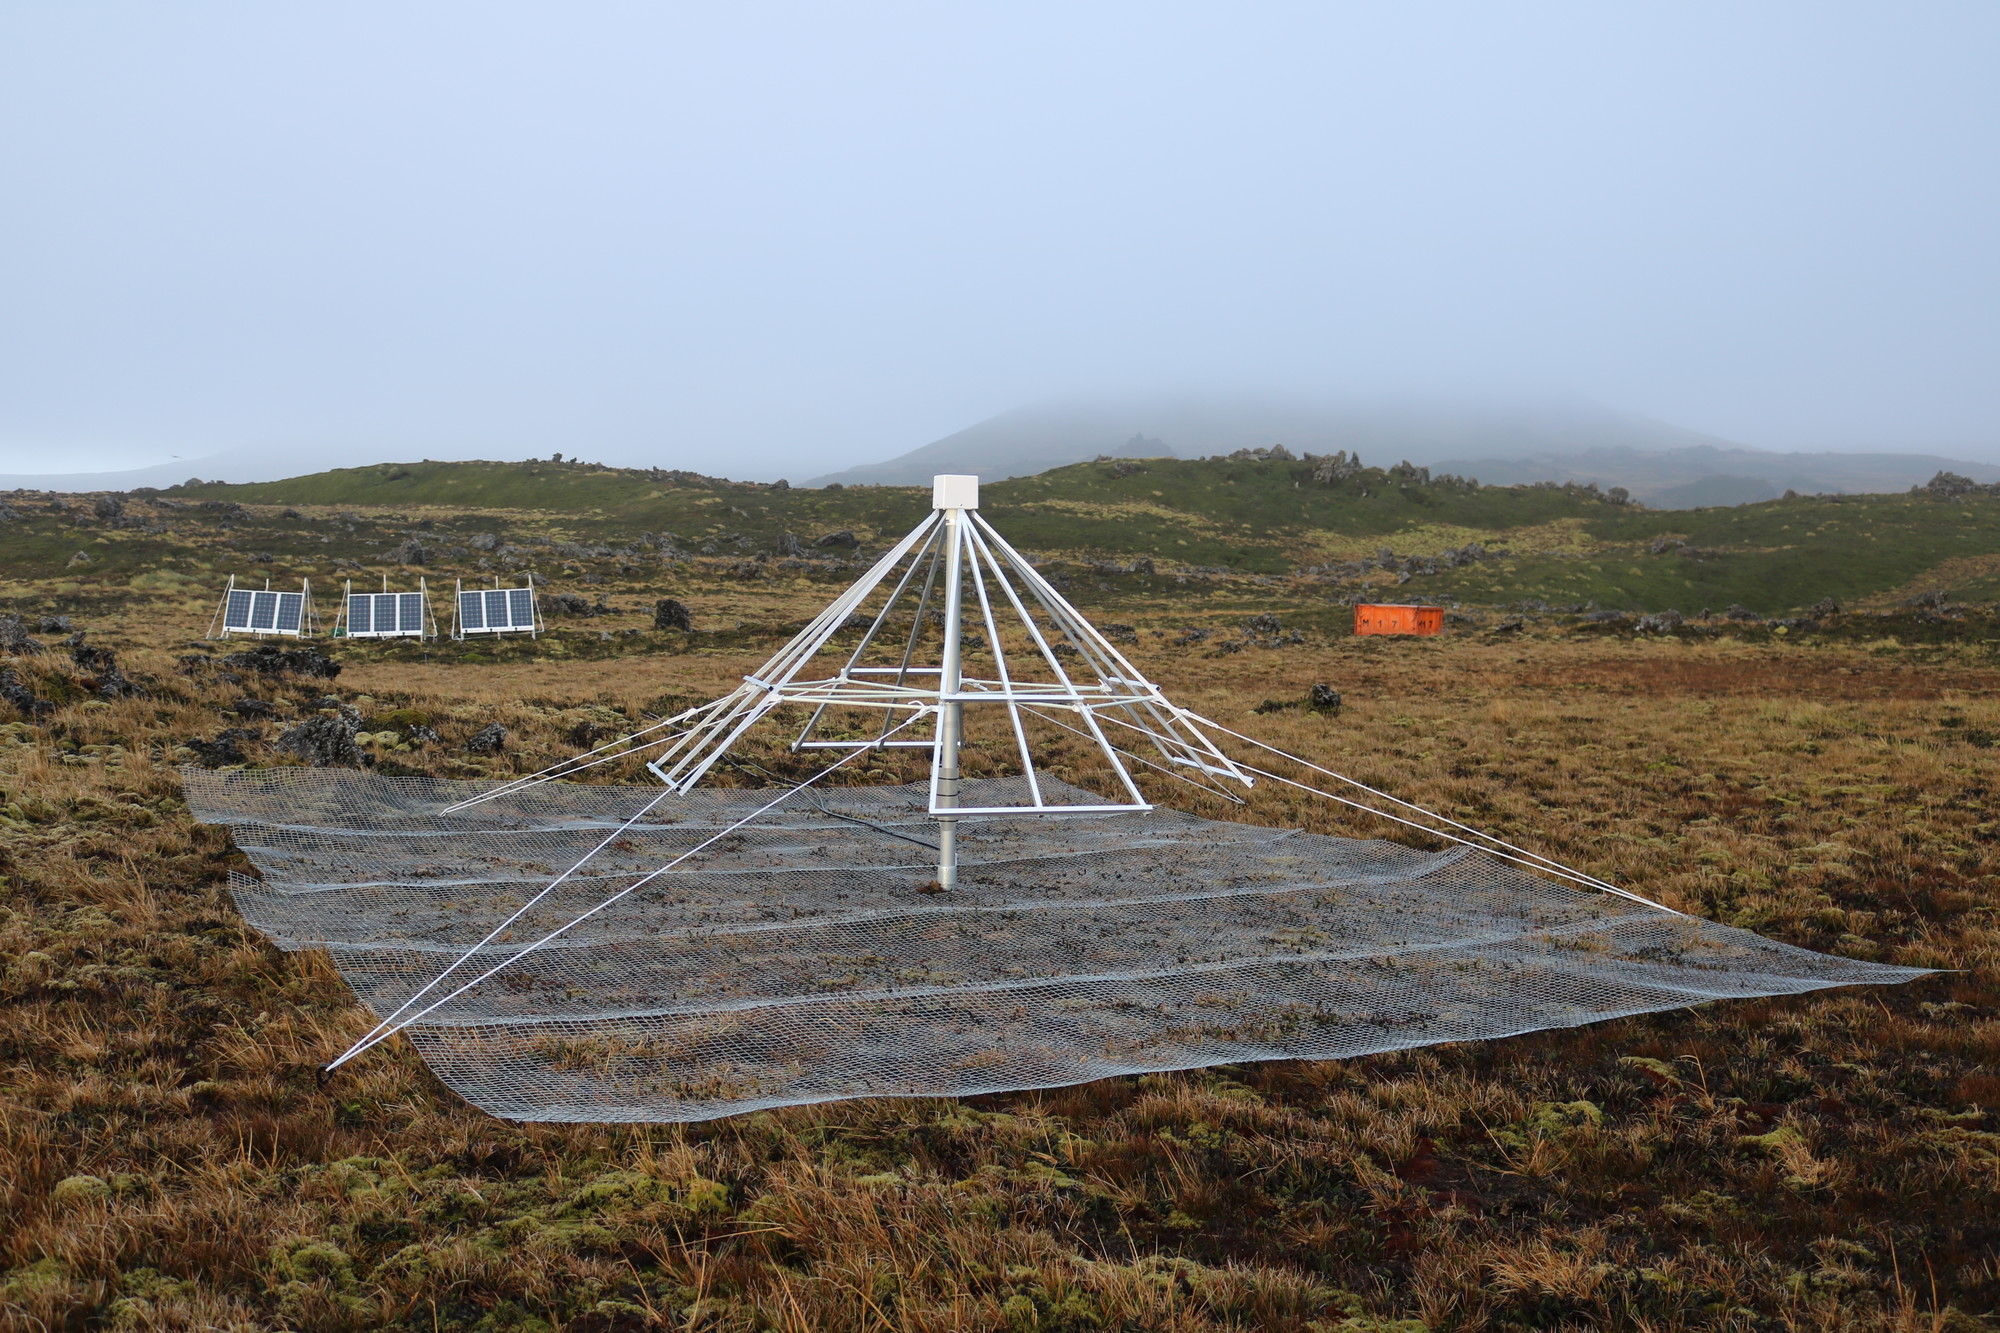
\includegraphics[width=0.7\linewidth]{Figures/autonomous.jpg}
    \caption{Single autonomous station pathfinder installed at the
      hydro shack site.  The system is powered by a bank of solar
      panels that are visible in the background.  \textcolor{red}{\bf
        Add command module and electronics glamor shots.}}
    \label{Fig:autonomous}
  \end{center}
\end{figure}

\begin{figure}
  \begin{center}
    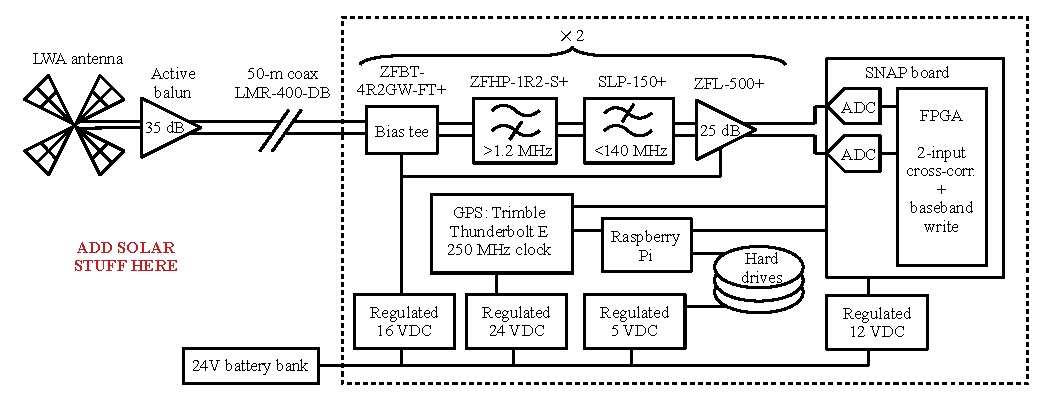
\includegraphics[width=\linewidth]{Figures/albatros_single_schematic/albatros_single_schematic.pdf}
    \caption{Schematic for the single autonomous station pathfinder.
      Data and RF connections are outlined in black, and power
      connections are outlined in red.  A dual-polarization LWA
      antenna, equipped with an active balun, is connected via 50-m
      coaxial cables to the back-end readout electronics, which are
      housed in a Faraday cage denoted by the dashed box.  Each of the
      two antenna inputs is passed to a second-stage electronics chain
      consisting of a bias tee, high- and low-pass filters, and
      amplifier.  The signals are digitized at 250~Msamp/s by a SNAP
      board, and the on-board FPGA is programmed with firmware that
      computes averaged auto- and cross-spectra, as well as
      channelized baseband.  A Raspberry Pi controls the SNAP board
      and saves the data products to a combination of an SD card and
      external hard drives.  Timing information is provided by a
      GPS-discipined clock.  Power to the system is provided solar
      panels that charges a 24-V battery bank, which is regulated down
      to several other output levels.}
    \label{Fig:Signal Chain}
  \end{center}
\end{figure}

\textcolor{red}{\bf Nivek?} \\

A single, autonomous station pathfinder was installed at the hydro
shack (\ang{46;52.205;}S, \ang{37;50.612;}E) in April 2019.

The final project (ALBATROS) will consist of autonomous antenna
stations that will map the low frequency sky. Since these experiments
are exploratory, they are taking steps towards achieving the future
objective of probing the Dark Ages.The ALBATROS stations (huts) will
be separated by baselines of \SI{\approx {20}}{km} as shown in
\autoref{Fig:Marion}. The two-element interferomentric pathfinder is
not yet operating autonomously, it uses the direct cross correlation
technique whereas the yet to be ALBATROS will write the lowest 10 - 20
MHz baseband to disk then gets correlated afterwards. One ALBATROS
fully autonomous station was deployed in Marion Island in April 2019
as shown in \autoref{Fig:autonomous}.

The single antenna analog signal chain is shown in \autoref{Fig:Signal
  Chain}. The components of the system are discussed in detail as per
the block diagram illustrated in \autoref{Fig:Signal Chain}. This
analog signal chain is an illustration of how the first autonomous
station is configured. There might be changes to the block diagram at
a later stage should there be a need to revise it for the stations.

% HCC: we probably don't need these figures below, or we can
% incorporate them as subfigs into other places

% \begin{figure}[h]
% 	\begin{center}
% 		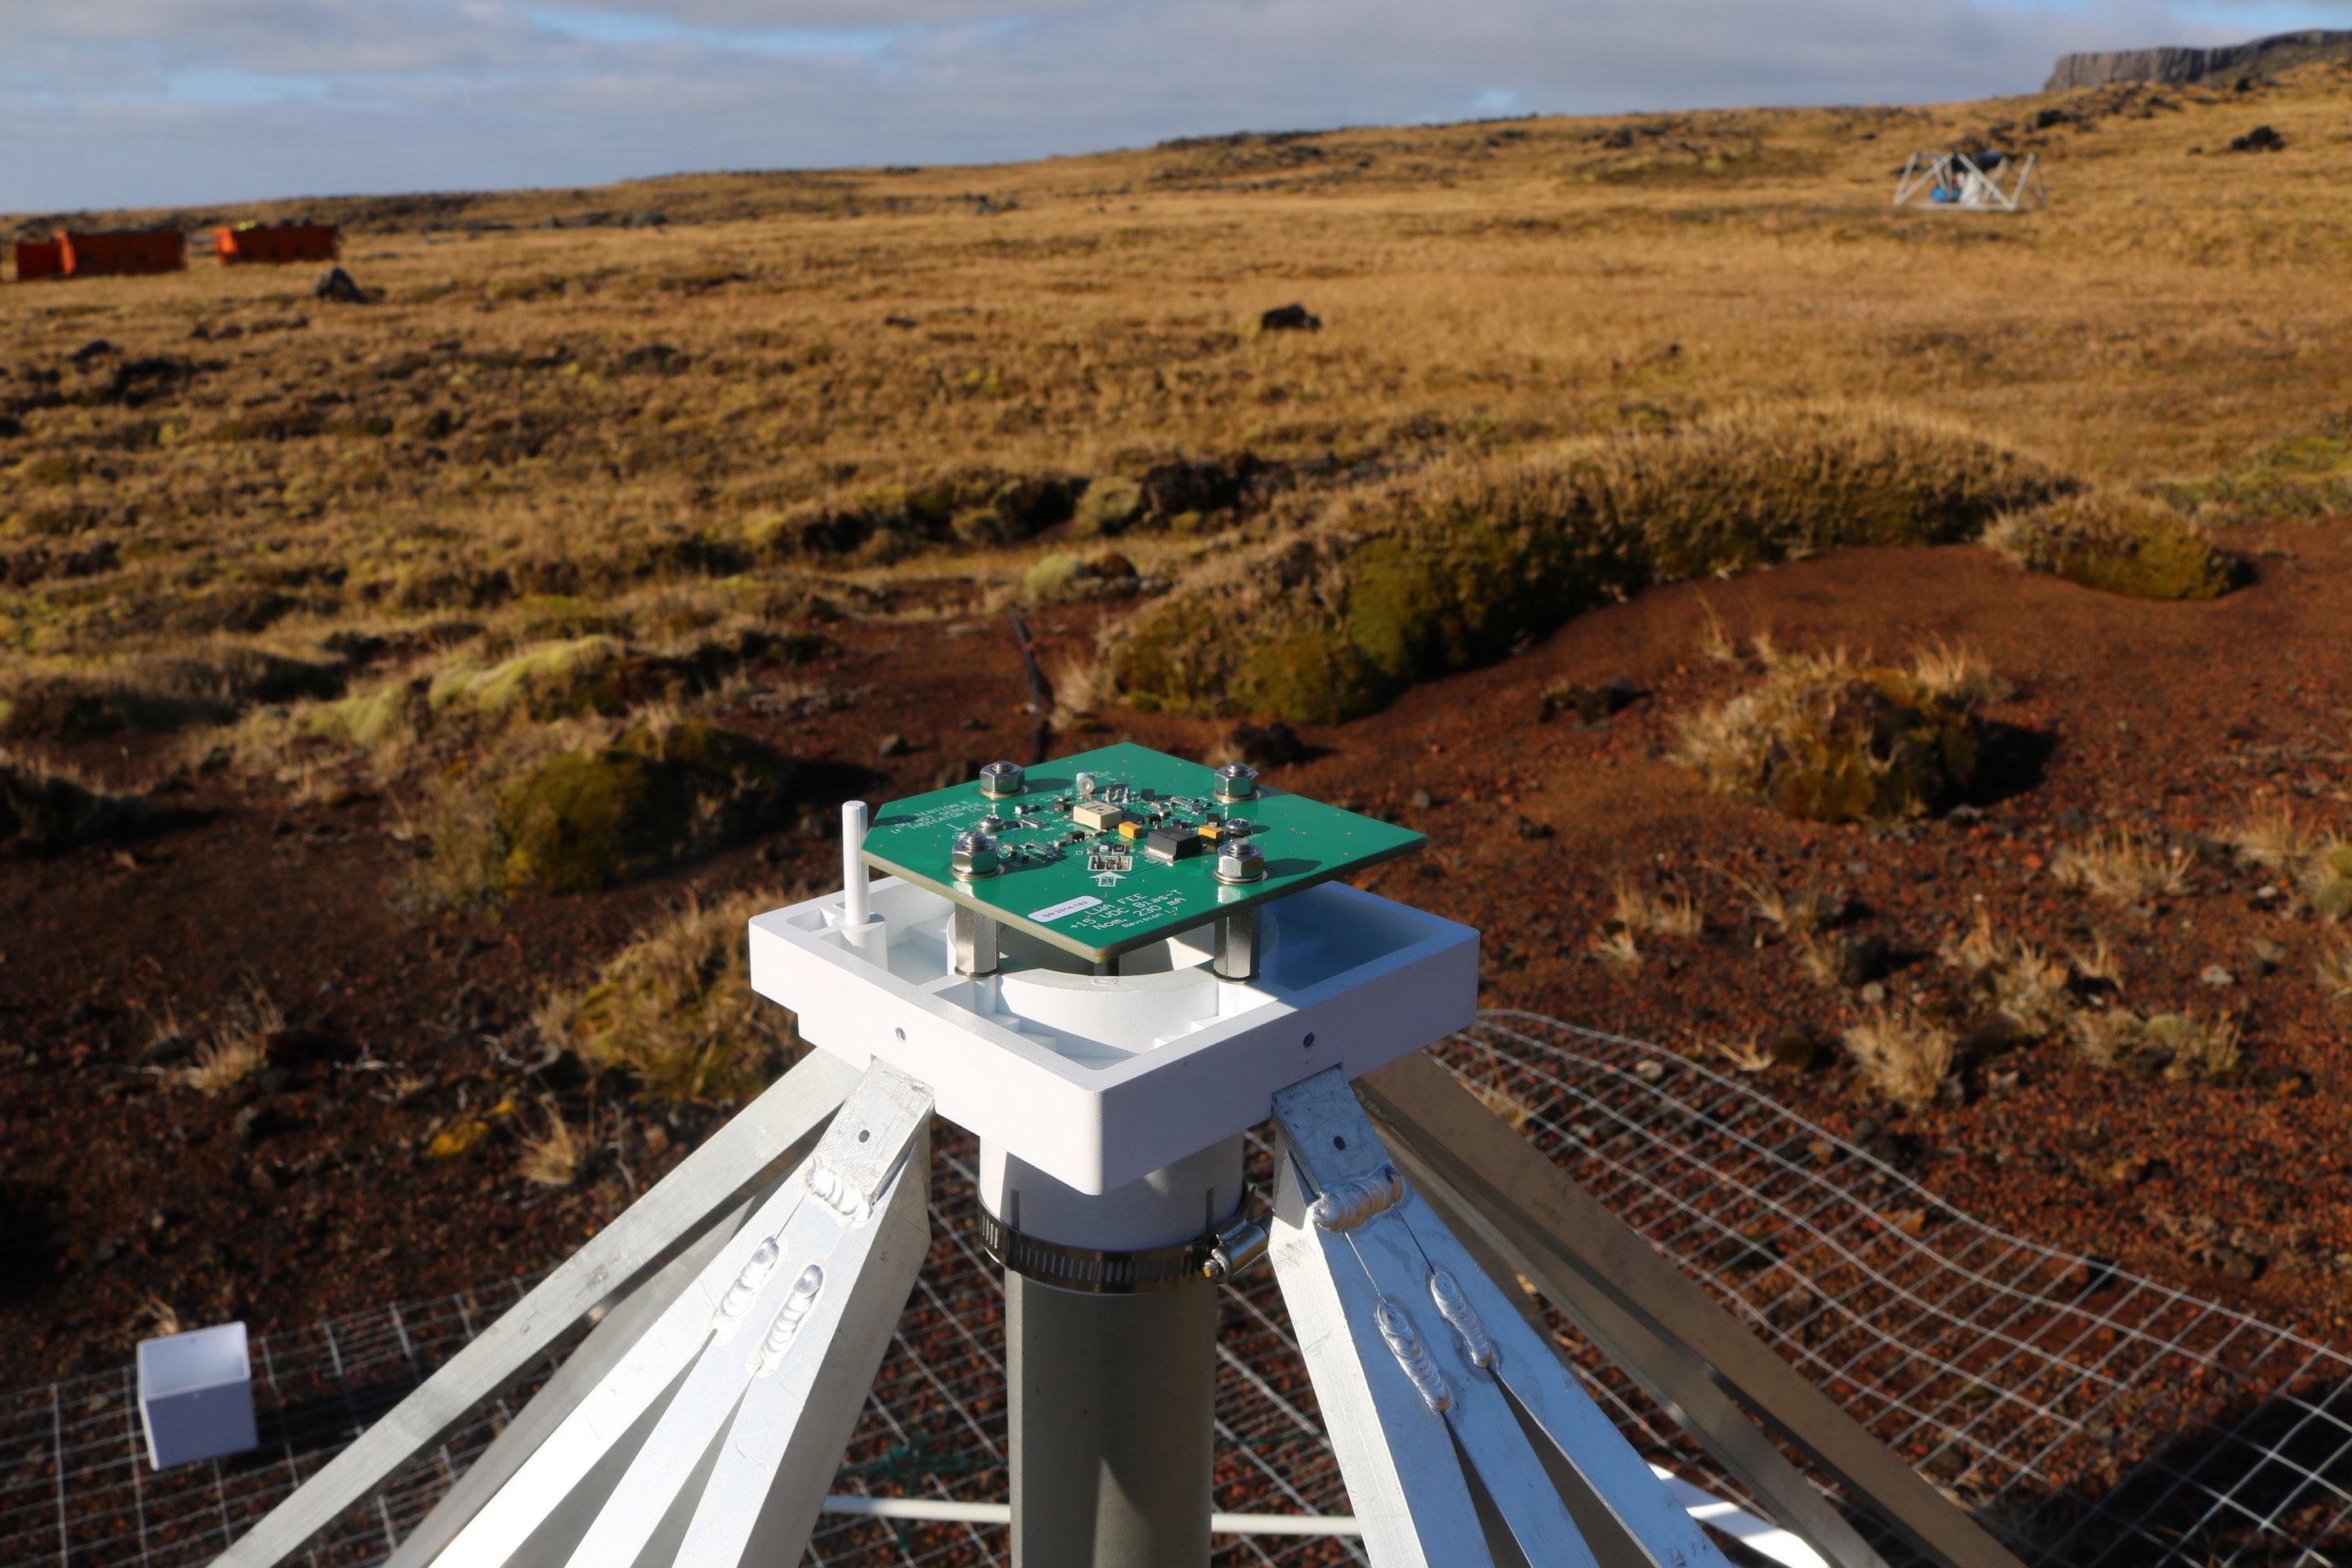
\includegraphics[width=0.5\linewidth]{Figures/balun.jpg}
% 		\caption{Unenclosed FEE mounted on the ALBATROS-EGG antenna supporting structure.} 
% 		\label{Fig:Balun}
% 	\end{center}
% \end{figure}
% 
% \begin{figure}[h]
% 	\begin{center}
% 		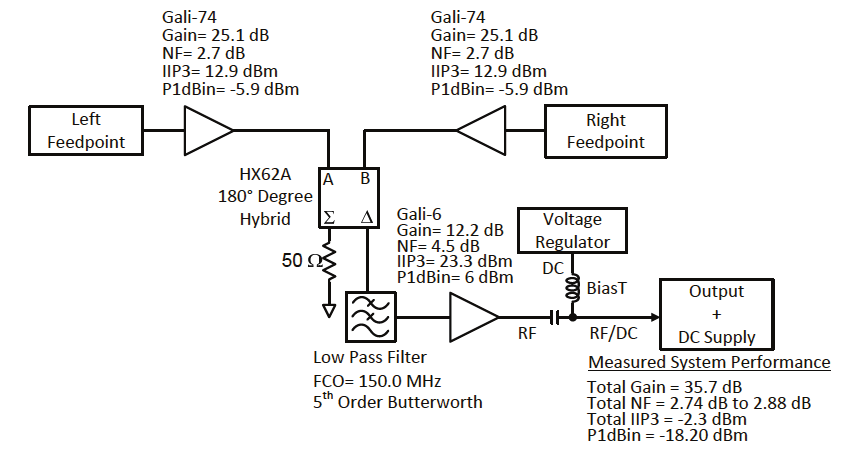
\includegraphics[width=0.7\linewidth]{Figures/Balun_Block.png}
% 		\caption{One Polarisation Block Diagram of the FEE \cite{2012PASP..124.1090H}}
% 		\label{Fig:Balun Schematic}
% 	\end{center}
% \end{figure}

\subsection{Readout electronics}
\textcolor{red}{\bf Nivek, Jon?} \\
Text here about one-bit stuff, pushing baseband through the RPi3,
clock requirements, data rates, etc.

\subsection{Correlation}
While the basics of 1-bit correlation are well known in the limit where the signal level is much lower than the noise, ALBATROS may well be in the high-signal regime.  We present the basics of 1-bit correlation here, and show that even in the high-signal limit, 1-bit correlation remains viable.
The fundamental output of a 1-bit correlator for real data is $x_{ij} \equiv \left < \tilde{E}_i \tilde{E}_j \right >$.  $ \tilde{E}_i$ is the quantized version of the underlying electric field $E_i$ where $ \tilde{E}_i=1$ for $E_i>0$ and $ \tilde{E}_i=-1$ for $E_i<0$.  Note that complex data can be handled as the combination of real components.  This output is non-linear in the underlying true signal and noise levels, since the output saturates at unity for perfectly correlated electric fields.  To get at the true sky signals, we will need to undo this nonlinearity (the so-called Van Vleck corrections).  For a 2-level correlator, the expected output can be related to the true signals as follows (Van Vleck \& Middleton, e.g. D'Addario):
\begin{eqnarray}
\label{eqn:1bit_output}
\left < \sin(\frac{\pi}{2}x_{ij})\right > = \frac{V_{ij}}{\sqrt{V_{ij}+N_i}\sqrt{V_{ij}+N_j}}
\end{eqnarray}
where $V_{ij}$ is the true visibility, and $V_{ij}+N_{i,j}$ is the total noise power measured by antennas $i$ and $j$.  Inverting this relation to get the true signal requires knowing the noise powers, which is not possible from the 1-bit data themselves.  However, the SNAP board calculates these power levels on timescales of a few seconds, much faster than the power levels change, and so by combining the single-station power measurements with the cross-station cross correlation, we will be able to derive the true sky visibilities.  

\begin{figure}
  \begin{center}
    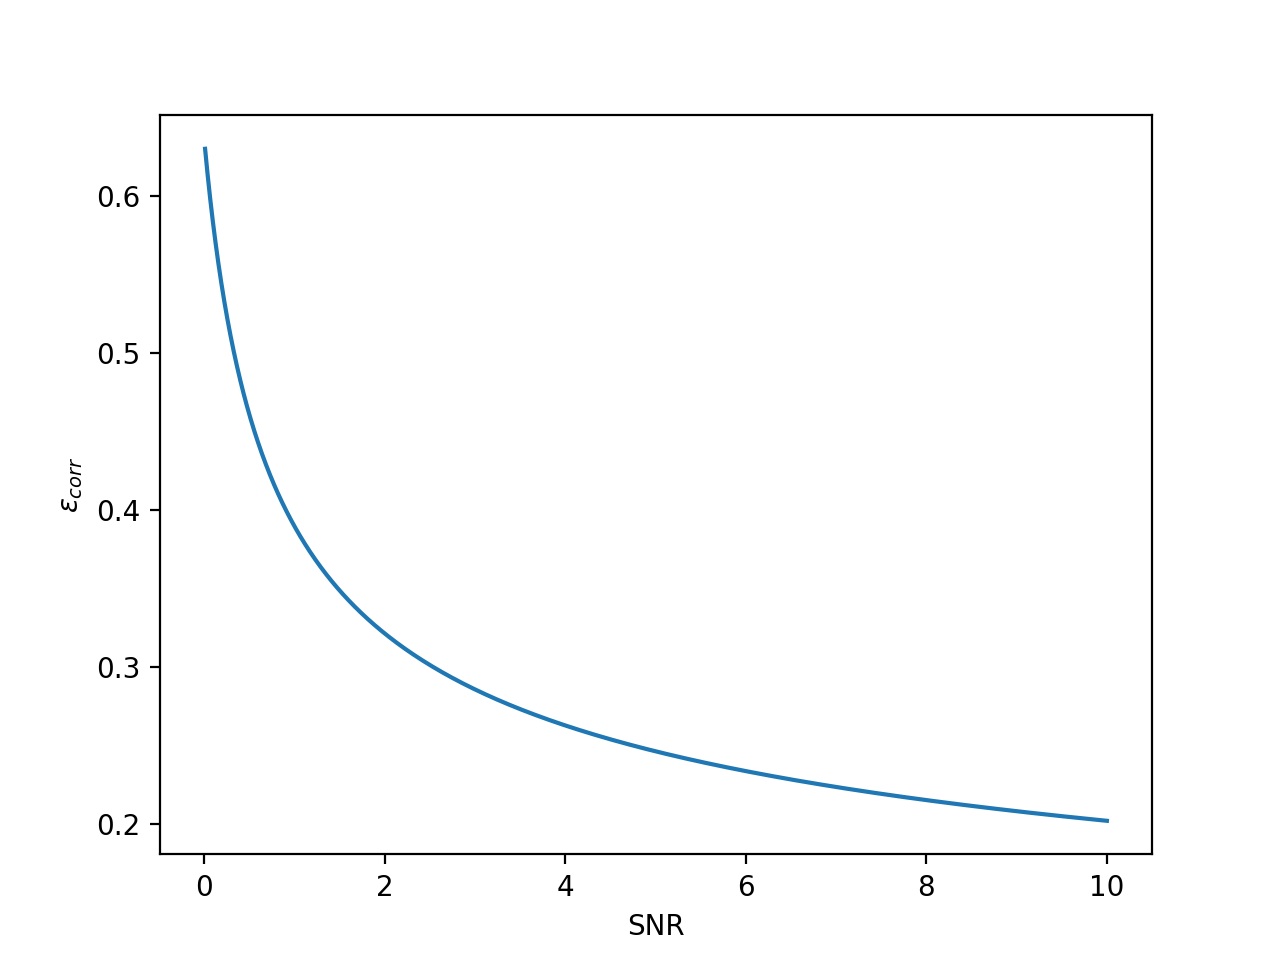
\includegraphics[width=0.7\linewidth]{Figures/corr_efficiency.png}
    \caption{Correlator efficiency $\epsilon_{corr}$ for a 1-bit correlator as a function of signal-to-noise ratio (SNR).  To get the expected SNR from a 1-bit correlator, multiply the SNR derived from the radiometer equation by $\epsilon_{corr}$.  For low SNR, the efficiency is $2/\pi \sim 0.64$, and it drops monotonically as the SNR increases.  The drop is relatively gentle, only changing by a factor of $\sim 2$ for SNR=2.  For baseline separations of many wavelengths, the correlated component of the electric field is likely to be a small fraction of the total power, so ALBATROS is unlikely to lose more than a factor of $\sim 2$ by using 1-bit correlation.}
    \label{Fig:1bit_efficiency}
    \end{center}
\end{figure}

One might worry that at high signal levels, the saturation of the 1-bit cross correlation would lead to the noise exploding.  In practice the rolloff in sensitivity is relatively mild, especially in the case of long baselines.  It can be expressed in terms of the correlator efficiency $\epsilon_{corr}$, which is defined to be the ratio of the measured signal-to-noise ratio to the ideal (infinite precision) SNR.  As seen in Figure \ref{fig:1bit_efficiency}, $\epsilon_{corr}$ only drops by a factor of $\sim$2 as the signal power goes from 0 to a few times the noise power.  We stress that the signal level is question is the part that correlates between the two antennas.  In the case of long baselines (where long means the fringe spacing is small compared to the primary beam/antenna response pattern) that are not dominated by a single bright source, the signal power will always be smaller than the noise power, and so $\epsilon_{corr}$ is unlikely to drop below $\sim$0.5\footnote{A quick estimate can be made by analogy to the behavior of dishes in the UV plane in the flat sky approximation.  While all power in the UV plane (plus any system noise) goes into an individual antenna's electric field, the correlated part only has contribution from the area in the UV plane within the width of the UV-space primary beam of the UV-space coordinate.  If the sky can be described as a Gaussian random field, in the most pessimistic case this is roughly the aperture filling factor of the antenna pair.  In our case, where the antennas are approximately dipolar, the filling factor will be the square of the wavelength over the baseline length.  As long as the baselines are several wavelengths or longer, the correlated power will be small, and the correlator efficiency will be close to the ideal 1-bit value of $\frac{2}{\pi}$.  


\subsection{Solar power system}
\textcolor{red}{\bf Nivek, Tankiso, Eamon?} \\
The power system of the ALBATROS-EGG uses generators to charge the batteries manually every once in a number of days. From the observation that has been made, the batteries take $\approx$ 2 days to discharge to a point where the system shuts down. Because of the weather conditions in Marion Island, an individual can sometimes be unable to go to the site to charge the batteries, which means that if the weather does not allow, the system can be shut down for a long period. Thus, a solar power system solution was introduced to the ALBATROS so that the system can continously run without having to be recharged manually and often.\\

The ALBATROS system is powered using \SI{24}{\volt} power which is stored and provided by two series-connected \SI{12}{\volt} deep-cycle lead-acid storage batteries. This power comes from the solar panel array consisting of nine flexible solar panels, each with a standard test condition capacity of \SI{110}{\watt}. The solar panel type is SunPower SPE-E-Flex-110. The panels are grouped in three parallel connected strings of three panels. Each group of three is mounted on its own structure. The panels include diodes to bypass shaded or defective cells, and also to prevent backwards current flow in the event an entire string of three panels is not illuminated while the others are producing power. \\

The Victron BlueSolar MPPT 50$\vert$35 charge controller outputs a data packet every second, to an Arduino based data logger, which controls a switch that determines when the rest of the system runs. It also converts the solar panel voltage to \SI{24}{\volt} to control the battery charging. The observed parameters are then stored to the raspberry pi.

\section{Preliminary observations}

\textcolor{red}{\bf NEED UPDATED AND NEW PLOTS, NEED VOLUNTEERS FOR THIS:
  \begin{itemize}
    \item{Improved waterfall plots from 2-element pathfinder}
    \item{Plot showing that the solar power works (sort of)}
    \item{Some sort of...data...plot for the autonomous station.  Can
      we say anything about baseband performance?}
  \end{itemize}
}
 
\autoref{Fig:auto} and \autoref{Fig:fringes} shows the initial results from the two interferometric array. These results are an encouraging factor to proceed with the development of the autonomous stations.\autoref{Fig:auto} shows the raw ALBATROS-EGG autospectra which where the waterfall plot was taken from one polarization (pol0) over an interval of 3 days. The Galaxy rising/setting is clearly visible in the structure. There are also ripples in frequency because of uncalibrated data, and the ripples arise from reflections in the cables. There is a qualitative difference between daytime and nighttime data and this shows that the contamination from shortwave radio drops off significantly at night, when the ionosphere becomes quieter.

\begin{figure}[h!]
	\begin{center}
		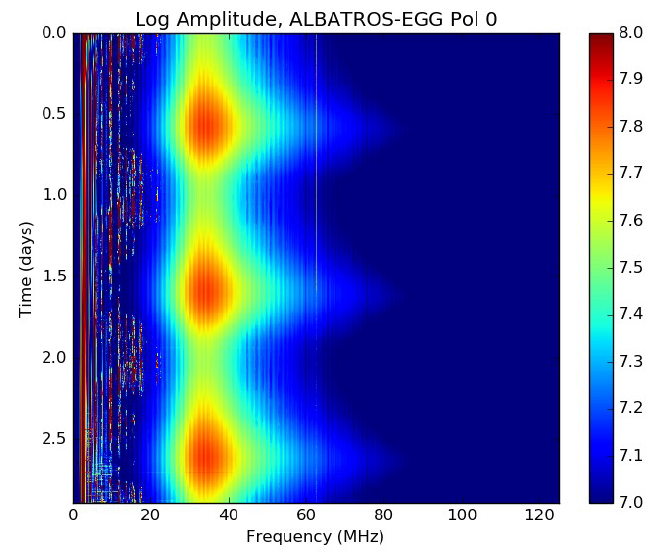
\includegraphics[width=0.8\linewidth]{Figures/Raw-ALBATROS-autospectra.PNG}
		\caption{Raw ALBATROS-EGG Autospectra}
		\label{Fig:auto}
	\end{center}
\end{figure}

\autoref{Fig:fringes} shows the first fringes that were detected by the the ALBATROS-EGG. It is dinstictly visible from \autoref{Fig:fringes} that fringes show recurrent structure down to a frequency of as low as 10 MHz without data processing or data cuts.

\begin{figure}[ht!]
	\begin{center}
		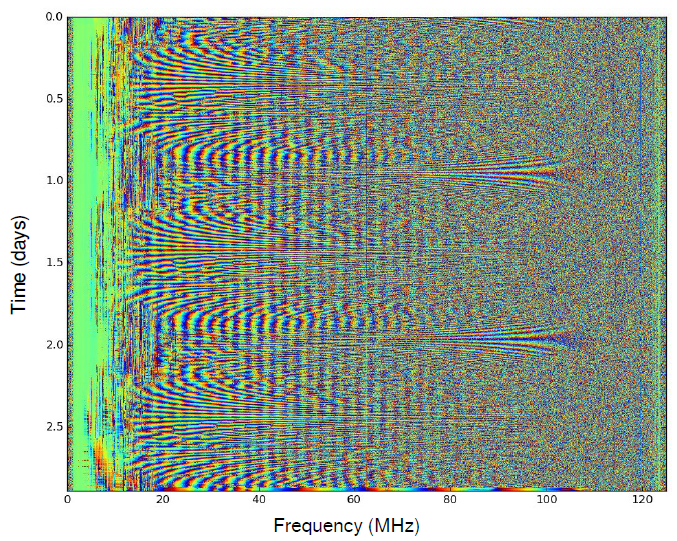
\includegraphics[width=0.7\linewidth]{Figures/First-fringes-of-ALBATROS-EGG.PNG}
		\caption{First Fringes from ALBATROS-EGG}
		\label{Fig:fringes}
	\end{center}
\end{figure}

% \section{Future Work}
	
\section*{Acknowledgments}

	
\begin{thebibliography}{9}

\bibitem[Alexander et al.(1975)]{1975A&A....40..365A} Alexander, J.~K., Kaiser, M.~L., Novaco, J.~C., et al.\ 1975, {\it aap\/}, {\bf 40}, 365

\bibitem[Chen {et al.}(2019)]{2019arXiv190710853C} Chen, X., Burns, J., Koopmans, L., {\it et al.} [2019], arXiv e-prints, arXiv:1907.10853

\bibitem[Eastwood et al.(2018)]{2018AJ....156...32E} Eastwood, M.~W., Anderson, M.~M., Monroe, R.~M., et al.\ 2018, {\it aj\/}, {\bf 156}, 32

\bibitem[Ellingson and Kramer (2004)]{Memo28} Ellingson, S.~W., {Kramer}, W.~T. \ 2004, {\it Long Wavelength Array Memo (28)}

\bibitem[George {et al.}(2018)] {article} George, M., Orchiston, W., Wielebinsk, R., {\it et al.} [2018], Journal of Astronomical History and Heritage, {\bf 21}, 37

\bibitem[Hicks et al.(2012)]{2012PASP..124.1090H} Hicks, B.~C., Paravastu-Dalal, N., Stewart, K.~P., et al.\ 2012, {\it pasp\/}, {\bf 124}, 1090

\bibitem[Koopmans {et al.}(2019)]{2019arXiv190804296K} Koopmans, L., Barkana, R., Bentum, M., {\it et al.} [2019], arXiv e-prints, arXiv:1908.04296

\bibitem[Liu {et al.}(2013)]{2013PhRvD..87d3002L} Liu, A., Pritchard, J.~R., Tegmark, M., {\it et al.} [2013], {\bf 87}, 043002

\bibitem[Philip {et al.}(2019)]{2019JAI.....850004P} Philip, L., Abdurashidova, Z., Chiang, H.~C., {\it et al.} [2019], Journal of Astronomical Instrumentation, {\bf 8}, 19500

\bibitem[Pober {et al.}(2014)]{2014ApJ...782...66P} Pober, J.~C., Liu, A., Dillon, J.~S., {\it et al.} [2014], {\bf 782}, 66

\bibitem[Ray et al.(2006)]{Memo35} Ray, P.~S., Ellingson, S.~W., Fisher R., {\it et al.} [2006] {\it Long Wavelength Array Memo (35)}

\bibitem[Roger et al.(1999)]{1999A&AS..137....7R} Roger, R.~S., Costain, C.~H., Landecker, T.~L., et al.\ 1999, {\it aaps\/}, {\bf 137}, 7

\bibitem[Weiler {et al.}(1988)]{1988A&A...195..372W} Weiler, K.~W., Johnston, K.~J., Simon, R.~S., {\it et al.} [1988], {\it aap\/}, {\bf 195}, 372






\end{thebibliography}
\end{document}
